\section{Pickup}
\label{pickup-project}

Electric guitars pickups are usually built by wrapping copper wire around magnets.
The working principle is based on the variation of magnetic field, created by the string
vibration. The vibration frequency of the string induces an electric signal on the output of the pickup \cite{pickup-work}
\cite{faraday-law}.

The designed pickup used the following main components:

{\begin{itemize}
  \item Base to assembly the set up magnet+coil
  \item 6 magnets
  \item Copper wire to wrap the magnets
  \item Cover to attach the set up on the guitar
\end{itemize}}

After some studies it was decided to build the pickup base using a 3D printer, due the
availability and reduced cost of this project. The model is showed on \autoref{3D-project}
and was projected using the AutoCAD software.

\begin{figure}[!htpb]
\centering
\caption{3D pickup base project}
\label{3D-project}
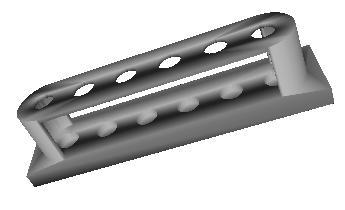
\includegraphics[scale=0.5]{images/pickup}
\legend{Source: Authors}
\end{figure}

There were two materials available to print the model, \textit{PLA} (Polylatic Acid) \cite{3d-materials}
and \textit{ABS} (Acrylonitrile Butadiene Styrene) \cite{3d-materials}. It was decided to print
the model on PLA because it attends the requisites of robustness of the project, is
faster to print and have a lower cost when compared to the other materials. \\
With the pickup base ready, coils were built by manually wrapping copper wire around
each magnet (\autoref{magnets}). Similar hexaphonic pickups can be found at the
market and researching about them gave the number of 500 turns as a reasonable amount
of wiring. \\
TODO -> EXPLAIN HOW TO TEST\\
TODO -> CALCULATE THE APROX. WIRE WIDTH BASED ON 500 turns\\

\begin{figure}[!htpb]
  \centering
  \caption{Magnets used on the project}
  \label{magnets}
  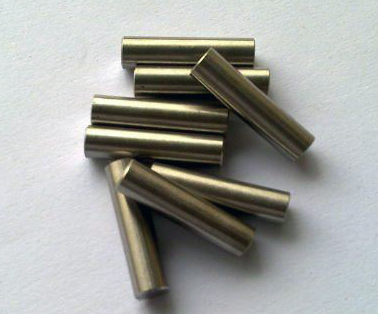
\includegraphics[scale=0.2]{images/magnets}
  \legend{Source: \citeonline{pickup-magnets}}
\end{figure}
